\documentclass[a4paper, 12pt]{article}
\usepackage{color}
\usepackage{scalerel}
\usepackage{tikz}
\usepackage{geometry}

\geometry{
		total = {160mm, 237mm},
		left = 25mm,
		right = 35mm,
		top = 30mm,
		bottom = 30mm,
	}

\usepackage{tabularx}
\usepackage{fancyhdr}
\usepackage{graphicx}
\usepackage{amssymb}
\usepackage{amsmath}
\usepackage{multicol}
\usepackage{graphicx}
\usepackage{wrapfig}
\usepackage{enumitem}
\usepackage{lastpage}
\usepackage{transparent}
\usepackage{cancel}
\usepackage{listings}

\newcommand{\ans}{\textbf{Jawab}:}


\begin{document}
\pagenumbering{gobble}
    \begin{tabular}{|lcl|}
     \hline
     Nama&:&Dhanar Agastya Rakalangi\\
     NRP&:&5002221075\\
     \hline
    \end{tabular}

    \begin{enumerate}
        \item Buatlah Coding dari UML berikut :
        \begin{figure}[h]
            \centering
            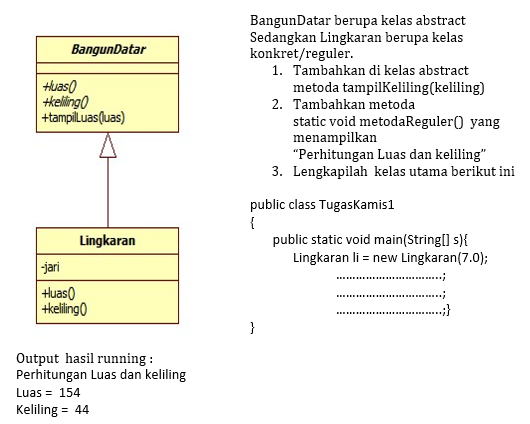
\includegraphics[width=1\linewidth]{No1.png}
        \end{figure}

        \newpage
        \ans
        
        \begin{lstlisting}[language=java, breaklines=true]
abstract class BangunDatar {
    abstract int luas();
    abstract int keliling();

    void tampilLuas(int luas) {
        System.out.println("Luas = " + luas);
    }

    void tampilKeliling(int keliling) {
        System.out.println("Keliling = " + keliling);
    }

    static void metodaReguler() {
        System.out.println("Perhitungan Luas dan keliling");
    }
}

class Lingkaran extends BangunDatar {
    int radius;

    Lingkaran(double radius) {
        this.radius = (int) radius;
    }
    int luas() {
        return (int) Math.round(Math.PI * radius * radius);
    }
    int keliling() {
        return (int) Math.round(2 * Math.PI * radius);
    }
    
public class TugasKamis1 {
    public static void main(String[] args) {
        Lingkaran obj = new Lingkaran(7.0);
        BangunDatar.metodaReguler();
        obj.tampilLuas(obj.luas());
        obj.tampilKeliling(obj.keliling());
    }
}

        \end{lstlisting}

        \newpage
        \item Betulkan kesalahan yang ada pada potongan coding berikut Dan tampilkan outputnya.
        \begin{figure}[h]
            \centering
            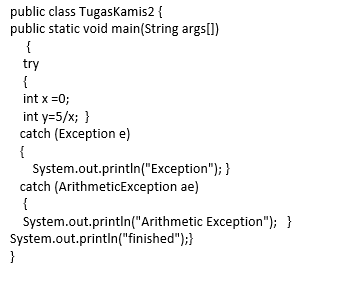
\includegraphics[width=0.6\linewidth]{No2.png}
        \end{figure}

        \newpage
        \ans
        \begin{lstlisting}[language=java, breaklines=true]
public class TugasKamis2 {
    public static void main(String args[]) {
        try {
            int x = 0;
            int y = 5 / x;
        } catch (ArithmeticException ae) {
            System.out.println("Arithmetic Exception");
        } catch (Exception e) {
            System.out.println("Exception");
        }
        System.out.println("finished");
    }
}

        \end{lstlisting}

        Output : \\
        Arithmetic Exception\\
        finished


        \newpage
        \item Lengkapilah program 
        \begin{figure}[h]
            \centering
            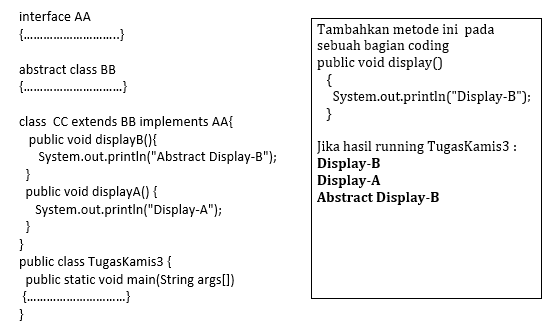
\includegraphics[width=1\linewidth]{No3.png}
        \end{figure}

        \newpage
        \ans
        \begin{lstlisting}[language=java , breaklines=true]
interface AA {
    void displayA();
}

abstract class BB {
    abstract void displayB();
}

class CC extends BB implements AA {
    public void displayB() {
        System.out.println("Abstract Display-B");
    }

    public void displayA() {
        System.out.println("Display-A");
    }

    public void display() {
        System.out.println("Display-B");
    }
}

public class TugasKamis3 {
    public static void main(String args[]) {
        CC obj = new CC();
        obj.display();
        obj.displayA();
        obj.displayB();
    }
}

        \end{lstlisting}
    \end{enumerate}

\end{document}